\chapter{Management Summary}

\instructions{
    
    Das Management Summary (auch Lay Summary) richtet sich an ein breites Publikum und an das
    Management, welches in der Regel über keine Fachkenntnisse im bearbeiteten Thema verfügen. Das
    Management Summary soll kurz und verständlich beschreiben, worum es bei der Arbeit geht und welche
    Ergebnisse erzielt wurden. Die Sprache soll knapp, klar und stark untergliedert sein. Der Umfang beträgt in
    der Regel 2-3 (max. 5) Seiten. Bilder sind hier im Gegensatz zum Abstract erwünscht.
    Beispiel Gliederung für Management Summary:
}

\section{Initial Situation}
Some functional languages, like Haskell, don't come with debuggers that are very user-friendly.
While Haskell does have a debugger,
it is fairly hard to use and it is not obvious,
how some information is obtained.

The debugger seems to jump around,
and when entering a function,
it seems like the context of the function call is lost.
It is not easy to see the values that are used when calling a function,
as they need to be fetched manually.

\begin{figure}[!ht]
    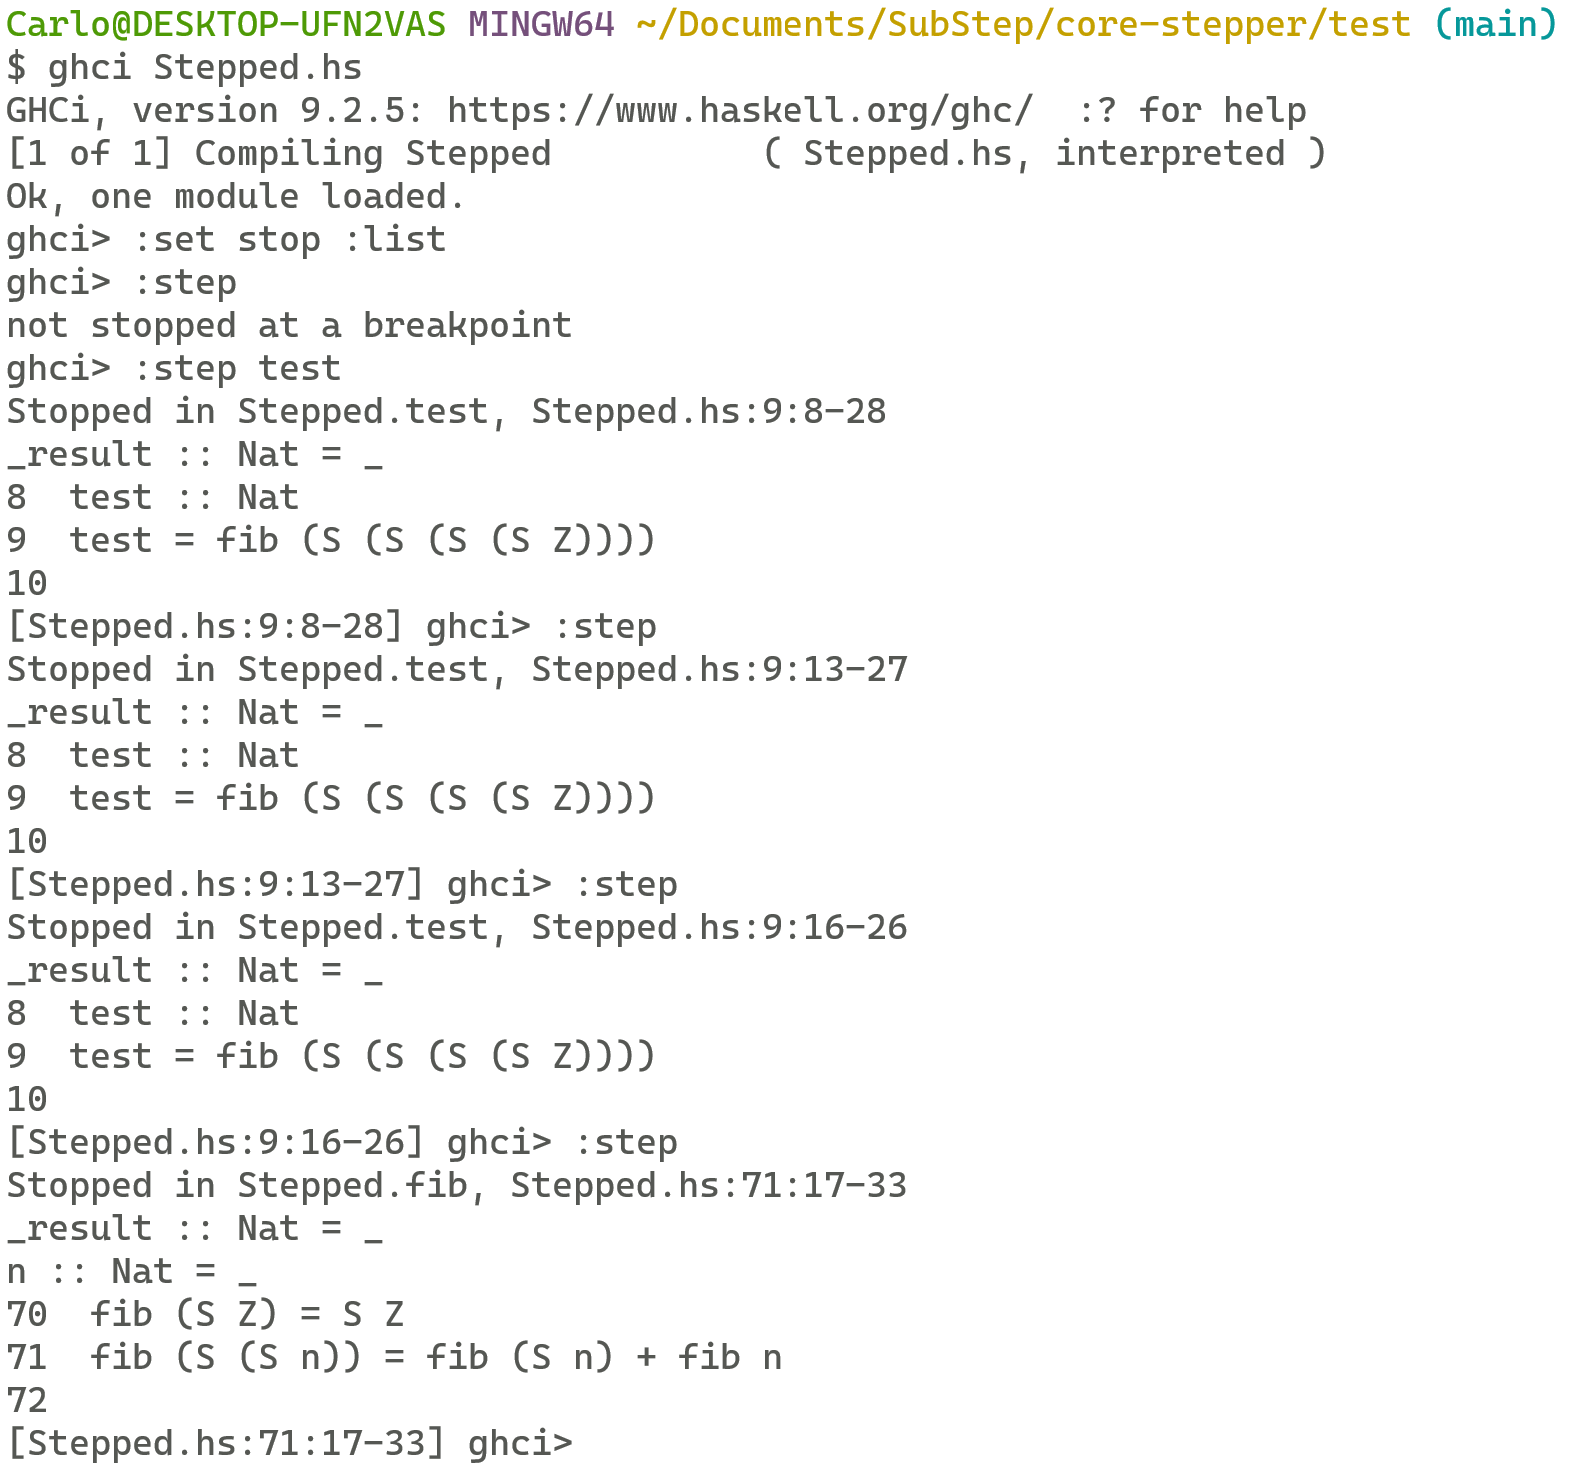
\includegraphics[width=0.75\textwidth]{resources/ghciDebug.png}
    \caption{Screenshot of the usage of the GHCi debugger. It is not clear what is going on and what the steps do.}
\end{figure}

To overcome these problems,
the Substitution Stepper was built as an alternative,
that makes it much easier to visualize the state of the program.

Some sketches of how the Substitution Stepper could work are shown in \ref*{ref:examplesSummary}

\begin{figure}[!ht]
    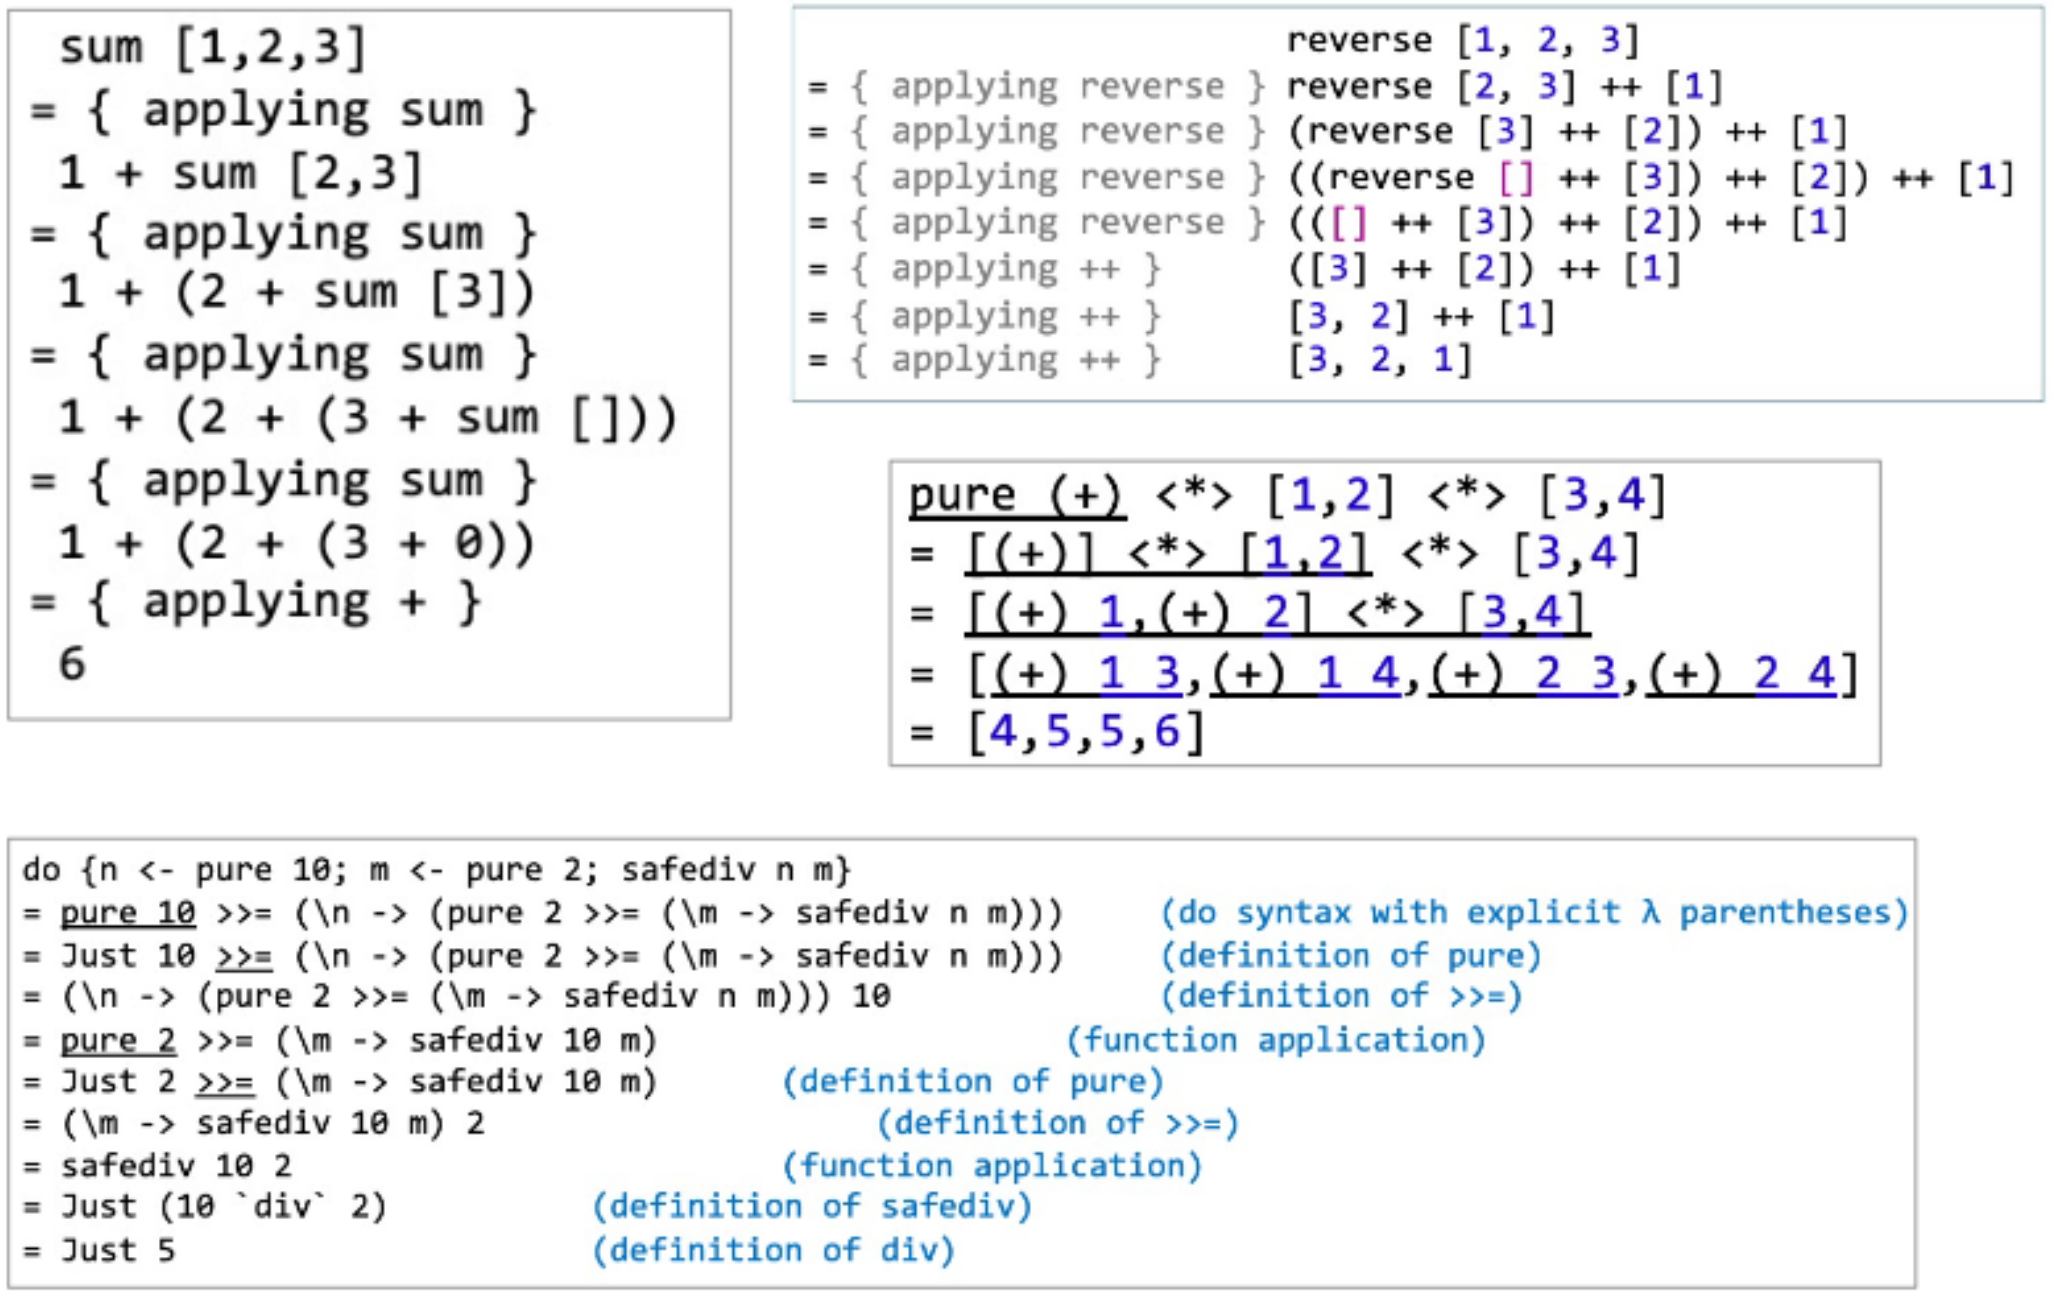
\includegraphics[width=0.75\textwidth]{resources/examples.PNG}
    \caption{Some examples of how the Substitution Stepper could work.}
    \label{fig:examplesSummary}
\end{figure}

\section{Implementation}
For the stepping the terms,
Haskell is compiled down to Core,
an intermediate langauge,
that simplifies many Haskell features to allow for better optimization and easier execution.

While it is easier to step Core,
it also comes with challenges translating it back to Haskell for the user.

\section{Results}
The result of this thesis is a command-line application that allows the stepping of Haskell code.
Most Haskell code can be stepped without problems,
however, there are some limitations,
since it is currently not possible to step functions using the Prelude,
which is the standard library for Haskell functions.

Besides the easier readability of the Substitution Stepper over the debugger,
it also comes with many useful features.
The user can step any term that they want in any order.
And there are different modes available,
also including an automatic mode that does the derivation automatically and shows the result when it's done.
